\chapter{scanf()}
\index{\CStandardLibrary!scanf()}
\label{label_scanf}

\RU{Теперь попробуем использовать scanf().}\EN{Now let's use scanf().}

% sections
\section{\RU{Простой пример}\EN{Simple example}}

\lstinputlisting{patterns/04_scanf/1_simple/ex1.c}

\RU{Использовать \scanf в наши времена для того, чтобы спросить у пользователя что-то\EMDASH{} 
не самая хорошая идея.
Но так мы проиллюстрируем передачу указателя на переменную типа \Tint.}
\EN{It's not clever to use \scanf for user interactions nowadays. 
But we can, however, illustrate passing a pointer to a variable of type \Tint.}

\subsection{\RU{Об указателях}\EN{About pointers}}
\index{\CLanguageElements!\Pointers}

\RU{Это одна из фундаментальных вещей в информатике.}\EN{Pointers are one of the fundamental concepts in computer science.}
\RU{Часто большой массив, структуру или объект передавать в другую функцию путем копирования данных невыгодно, 
а передать адрес массива, структуры или объекта куда проще.}
\EN{Often, passing a large array, structure or object as an argument to another function is too expensive, 
while passing their address is much cheaper.}
\RU{К тому же, если вызываемая функция (\gls{callee}) должна изменить что-то в этом большом массиве или структуре,
то возвращать её полностью так же абсурдно.}
\EN{In addition if the \gls{callee} function needs to modify something in the large array or structure received as a parameter and return back the entire structure then the situation is close to absurd.}
\RU{Так что самое простое, что можно сделать, это передать в функцию-\gls{callee} адрес массива или структуры,
и пусть \gls{callee} что-то там изменит.}
\EN{So the simplest thing to do is to pass the address of the array or structure to the \gls{callee} function,
and let it change what needs to be changed.}

\RU{Указатель в}\EN{A pointer in} \CCpp\RU{\EMDASH{}это просто адрес какого-либо места в памяти.}
\EN{ is simply an address of some memory location.}

\index{x86-64}
\RU{В x86 адрес представляется в виде 32-битного числа (т.е. занимает 4 байта), а в x86-64 как 64-битное число 
(занимает 8 байт).}
\EN{In x86, the address is represented as a 32-bit number (i.e., it occupies 4 bytes), while in x86-64 it is a 64-bit number (occupying 8 bytes).}
\RU{Кстати, отсюда негодование некоторых людей, связанное с переходом на x86-64\EMDASH{}на этой архитектуре все указатели
занимают в 2 раза больше места, в том числе и в ``дорогой'' кэш-памяти.}
\EN{By the way, that is the reason behind some people's indignation related to switching to x86-64\EMDASH{}all pointers
in the x64-architecture require twice as much space, including cache memory, which is ``expensive'' place.}

\index{\CStandardLibrary!memcpy()}
\RU{При некотором упорстве можно работать только с безтиповыми указателями (\TT{void*})}\EN{
It is possible to work with untyped pointers only, given some effort}; \RU{например,}\EN{e.g.} 
\RU{стандартная функция Си}\EN{the standard C function} \TT{memcpy()},
\RU{копирующая блок из одного места памяти в другое}\EN{that copies a block from one memory location to another}, 
\RU{принимает на вход 2 указателя типа}\EN{takes 2 pointers of type } \TT{void*}\EN{ as arguments}, 
\RU{потому что нельзя
заранее предугадать, какого типа блок вы собираетесь копировать. 
Для копирования тип данных не важен, важен только размер блока.}
\EN{since it is impossible to predict the type of the data you would like to copy. 
Data types are not important, only the block size matters.}

\RU{Также указатели широко используются, когда функции нужно вернуть более одного значения}
\EN{Pointers are also widely used when a function needs to return more than one value}
(\RU{мы ещё вернемся к этому в будущем}\EN{we are going to get back to this later}
\ifx\LITE\undefined
~(\myref{label_pointers})
\fi
).
\RU{Функция }\IT{scanf()}\RU{\EMDASH{}это как раз такой случай}\EN{ is such a case}. 
\RU{Помимо того, что этой функции нужно показать, сколько значений
было прочитано успешно, ей ещё и нужно вернуть сами значения.}
\EN{Besides the fact that the function needs to indicate how many values were successfully read, 
it also needs to return all these values.}

\RU{Тип указателя в}\EN{In} \CCpp \RU{нужен для проверки типов на стадии компиляции.}
\EN{the pointer type is only needed for compile-time type checking.}
\RU{Внутри, в скомпилированном коде, никакой информации о типах указателей нет вообще.}
\EN{Internally, in the compiled code there is no information about pointer types at all.}

\subsection{x86}

\subsubsection{MSVC}

\RU{Что получаем на ассемблере, компилируя в MSVC 2010:}
\EN{Here is what we get after compiling with MSVC 2010:}

\lstinputlisting{patterns/04_scanf/1_simple/ex1_MSVC.asm.\LANG}

\RU{Переменная \TT{x} является локальной.}\EN{\TT{x} is a local variable.} 

\RU{По стандарту \CCpp она доступна только из этой же функции и нигде более. 
Так получилось, что локальные переменные располагаются в стеке. 
Может быть, можно было бы использовать и другие варианты, но в x86 это традиционно так.}
\EN{According to the \CCpp standard it must be visible only in this function and not from any other external scope. 
Traditionally, local variables are stored on the stack. 
There are probably other ways to allocate them, but in x86 that is the way it is.}

\index{x86!\Instructions!PUSH}
\RU{Следующая после пролога инструкция \TT{PUSH ECX} не ставит своей целью сохранить 
значение регистра \ECX. 
(Заметьте отсутствие соответствующей инструкции \TT{POP ECX} в конце функции).}
\EN{The goal of the instruction following the function prologue, \TT{PUSH ECX}, is not to save the \ECX state 
(notice the absence of corresponding \TT{POP ECX} at the function's end).}

\RU{Она на самом деле выделяет в стеке 4 байта для хранения \TT{x} в будущем.} 
\EN{In fact it allocates 4 bytes on the stack for storing the \TT{x} variable.} 

\label{stack_frame}
\index{\Stack!\RU{Стековый фрейм}\EN{Stack frame}}
\index{x86!\Registers!EBP}
\RU{Доступ к \TT{x} будет осуществляться при помощи объявленного макроса \TT{\_x\$} 
(он равен -4) и регистра \EBP указывающего на текущий фрейм.}
\EN{\TT{x} is to be accessed with the assistance of the \TT{\_x\$} macro 
(it equals to -4) and the \EBP register pointing to the current frame.}

\RU{Во всё время исполнения функции \EBP указывает на текущий \glslink{stack frame}{фрейм} и через \TT{EBP+смещение}
можно получить доступ как к локальным переменным функции, так и аргументам функции.} 
\EN{Over the span of the function's execution, \EBP is pointing to the current \gls{stack frame} 
making it possible to access local variables and function arguments via \TT{EBP+offset}.}

\index{x86!\Registers!ESP}
\RU{Можно было бы использовать \ESP, но он во время исполнения функции часто меняется, а это не удобно. 
Так что можно сказать, что \EBP это \IT{замороженное состояние} \ESP на момент начала исполнения функции.}
\EN{It is also possible to use \ESP for the same purpose, although that is not very convenient since it changes frequently.
The value of the \EBP could be perceived as a \IT{frozen state} of the value in \ESP at the start of the function's execution.}

% FIXME1 это уже было в 02_stack?
\RU{Разметка типичного стекового \glslink{stack frame}{фрейма} в 32-битной среде}%
\EN{Here is a typical \gls{stack frame} layout in 32-bit environment}:

\begin{center}
\begin{tabular}{ | l | l | }
\hline
\dots & \dots \\
\hline
EBP-8 & \RU{локальная переменная}\EN{local variable} \#2, \MarkedInIDAAs{} \TT{var\_8} \\
\hline
EBP-4 & \RU{локальная переменная}\EN{local variable} \#1, \MarkedInIDAAs{} \TT{var\_4} \\
\hline
EBP & \RU{сохраненное значение}\EN{saved value of} \EBP \\
\hline
EBP+4 & \RU{адрес возврата}\EN{return address} \\
\hline
EBP+8 & \argument \#1, \MarkedInIDAAs{} \TT{arg\_0} \\
\hline
EBP+0xC & \argument \#2, \MarkedInIDAAs{} \TT{arg\_4} \\
\hline
EBP+0x10 & \argument \#3, \MarkedInIDAAs{} \TT{arg\_8} \\
\hline
\dots & \dots \\
\hline
\end{tabular}
\end{center}

\RU{У функции \scanf в нашем примере два аргумента.}\EN{The \scanf function in our example has two arguments.}

\RU{Первый~--- указатель на строку, содержащую \TT{\%d} и второй~--- адрес переменной \TT{x}.} 
\EN{The first one is a pointer to the string containing \TT{\%d} and the second is the address of the \TT{x} variable.} 

\index{x86!\Instructions!LEA}
\RU{Вначале адрес \TT{x} помещается в регистр \EAX при помощи инструкции \TT{lea eax, DWORD PTR \_x\$[ebp]}.}
\EN{First, the \TT{x} variable's address is loaded into the \EAX register by the \TT{lea eax, DWORD PTR \_x\$[ebp]} instruction}

\ifx\LITE\undefined
\RU{Инструкция \LEA означает \IT{load effective address}, и часто используется для формирования адреса чего-либо}
\EN{\LEA stands for \IT{load effective address}, and is often used for forming an address}
~(\myref{sec:LEA}).
\fi

\RU{Можно сказать, что в данном случае \LEA просто помещает в \EAX результат суммы значения в регистре 
\EBP и макроса \TT{\_x\$}.}
\EN{We could say that in this case \LEA simply stores the sum of the \EBP register value and the \TT{\_x\$} macro in the \EAX register.}

\RU{Это тоже что и}\EN{This is the same as} \TT{lea eax, [ebp-4]}.

\RU{Итак, от значения \EBP отнимается 4 и помещается в \EAX.
Далее значение \EAX заталкивается в стек и вызывается \scanf.}
\EN{So, 4 is being subtracted from the \EBP register value and the result is loaded in the \EAX register.
Next the \EAX register value is pushed into the stack and \scanf is being called.}

\RU{После этого вызывается \printf. Первый аргумент вызова строка:} 
\EN{\printf is being called after that with its first argument --- a pointer to the string:} \TT{You entered \%d...\textbackslash{}n}.

\RU{Второй аргумент: \TT{mov ecx, [ebp-4]}. Эта инструкция помещает в \ECX не адрес переменной \TT{x}, 
а её значение.}
\EN{The second argument is prepared with: \TT{mov ecx, [ebp-4]}.
The instruction stores the \TT{x} variable value and not its address, in the \ECX register.}

\RU{Далее значение \ECX заталкивается в стек и вызывается \printf.}
\EN{Next the value in the \ECX is stored on the stack and the last \printf is being called.}

\ifdefined\IncludeOlly
\clearpage
\subsection{MSVC + \olly}
\index{\olly}

\RU{Попробуем этот же пример в}\EN{Let's try this example in} \olly.
\RU{Загружаем, нажимаем F8 (\stepover) до тех пор, пока не окажемся в своем исполняемом файле,
а не в}\EN{Let's load it and keep pressing F8 (\stepover) until we reach our executable file
instead of} \TT{ntdll.dll}.
\RU{Прокручиваем вверх до тех пор, пока не найдем \main}\EN{Scroll up until \main appears}.
\RU{Щелкаем на первой инструкции (\TT{PUSH EBP}), нажимаем F2 (\IT{set a breakpoint}), 
затем F9 (\IT{Run}) и точка останова срабатывает на начале \main.}
\EN{Click on the first instruction (\TT{PUSH EBP}), press F2 (\IT{set a breakpoint}), 
then F9 (\IT{Run}).
The breakpoint will be triggered when \main begins.}

\RU{Трассируем до того места, где готовится адрес переменной $x$}%
\EN{Let's trace to the point where the address of the variable $x$ is calculated}:

\begin{figure}[H]
\centering
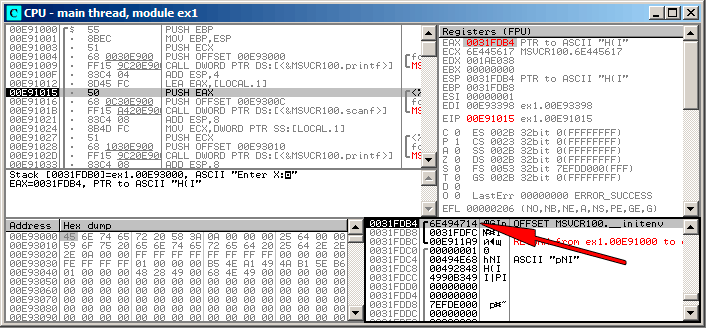
\includegraphics[scale=\FigScale]{patterns/04_scanf/1_simple/ex1_olly_1.png}
\caption{\olly: \RU{вычисляется адрес локальной переменной}\EN{The address of the local variable is calculated}}
\label{fig:scanf_ex1_olly_1}
\end{figure}

\RU{На \EAX в окне регистров можно нажать правой кнопкой и далее выбрать}
\EN{Right-click the \EAX in the registers window and then select} \q{Follow in stack}.
\RU{Этот адрес покажется в окне стека.}
\EN{This address will appear in the stack window.}
\RU{Смотрите, это переменная в локальном стеке. Там дорисована красная стрелка}%
\EN{The red arrow has been added, pointing to the variable in the local stack}.
\RU{И там сейчас какой-то мусор}\EN{At that moment this location contains some garbage} (\TT{0x6E494714}).
\RU{Адрес этого элемента стека сейчас, при помощи \PUSH запишется в этот же стек рядом}%
\EN{Now with the help of \PUSH instruction the address of this stack element is going to be stored to the same stack on the next position}.
\RU{Трассируем при помощи F8 вплоть до конца исполнения \scanf}\EN{Let's trace with F8 until the \scanf execution completes}.
\RU{А пока \scanf исполняется, в консольном окне, вводим, например, 123}%
\EN{During the \scanf execution, we input, for example, 123, in the console window}:

\begin{figure}[H]
\centering
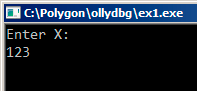
\includegraphics[scale=\NormalScale]{patterns/04_scanf/1_simple/ex1_olly_2.png}
\caption{\RU{Ввод пользователя в консольном окне}\EN{User input in the console window}}
\label{fig:scanf_ex1_olly_2}
\end{figure}

\clearpage
\RU{Вот тут }\scanf \RU{отработал}\EN{completed its execution already}:

\begin{figure}[H]
\centering
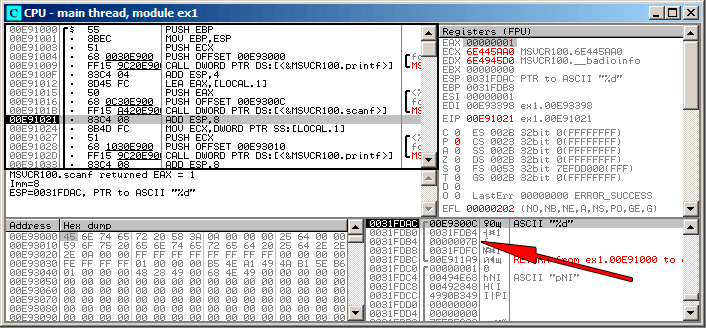
\includegraphics[scale=\FigScale]{patterns/04_scanf/1_simple/ex1_olly_3.png}
\caption{\olly: \scanf \RU{исполнилась}\EN{executed}}
\label{fig:scanf_ex1_olly_3}
\end{figure}

\scanf \RU{вернул}\EN{returns} 1 \InENRU \EAX, \RU{что означает, что он успешно прочитал одно 
значение}\EN{which implies that it has read successfully one value}.
\RU{В наблюдаемом нами элементе стека теперь}\EN{If we look again at the stack element corresponding to the local variable it now contains} \TT{0x7B} (123).

\clearpage
\RU{Чуть позже это значение копируется из стека в регистр \ECX и передается в \printf}
\EN{Later this value is copied from the stack to the \ECX register and passed to \printf}:

\begin{figure}[H]
\centering
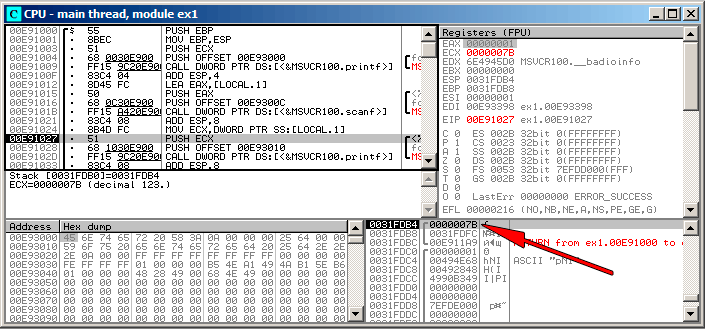
\includegraphics[scale=\FigScale]{patterns/04_scanf/1_simple/ex1_olly_4.png}
\caption{\olly: \RU{готовим значение для передачи в}\EN{preparing the value for passing to} \printf}
\label{fig:scanf_ex1_olly_4}
\end{figure}

\fi

\ifdefined\IncludeGCC
\subsubsection{GCC}

\RU{Попробуем тоже самое скомпилировать в Linux при помощи GCC 4.4.1:}
\EN{Let's try to compile this code in GCC 4.4.1 under Linux:}

\lstinputlisting{patterns/04_scanf/1_simple/ex1_GCC.asm}

\index{puts() \RU{вместо}\EN{instead of} printf()}
\RU{GCC заменил первый вызов \printf на \puts. Почему это было сделано, 
уже было описано ранее~(\myref{puts}).}
\EN{GCC replaced the \printf call with call to \puts. The reason for this was explained in ~(\myref{puts}).}

% TODO: rewrite
%\RU{Почему \scanf переименовали в \TT{\_\_\_isoc99\_scanf}, я честно говоря, пока не знаю.}
%\EN{Why \scanf is renamed to \TT{\_\_\_isoc99\_scanf}, I do not know yet.}
% 
% Apparently it has to do with the ISO c99 standard compliance. By default GCC allows specifying a standard to adhere to.
% For example if you compile with -std=c89 the outputted assmebly file will contain scanf and not __isoc99__scanf. I guess current GCC version adhares to c99 by default.
% According to my understanding the two implementations differ in the set of suported modifyers (See printf man page)


\RU{Далее всё как и прежде~--- параметры заталкиваются через стек при помощи \MOV.}
\EN{As in the MSVC example---the arguments are placed on the stack using the \MOV instruction.}
\fi

\subsubsection{\RU{Кстати}\EN{By the way}}

\RU{Кстати, этот простой пример иллюстрирует то обстоятельство, что компилятор преобразует
список выражений в \CCpp-блоке просто в последовательный набор инструкций.}
\EN{By the way, this simple example is a demonstration of the fact that compiler translates
list of expressions in \CCpp-block into sequential list of instructions.}
\RU{Между выражениями в \CCpp ничего нет, и в итоговом машинном коде между ними тоже ничего нет, 
управление переходит от одной инструкции к следующей за ней.}
\EN{There are nothing between expressions in \CCpp, and so in resulting machine code, 
there are nothing between, control flow slips from one expression to the next one.}

\subsection{x64}

\index{x86-64}
\RU{Всё то же самое, только используются регистры вместо стека для передачи аргументов функций}%
\EN{The picture here is similar with the difference that the registers, rather than the stack, are used for arguments passing}.

\subsubsection{MSVC}

\lstinputlisting[caption=MSVC 2012 x64]{patterns/04_scanf/1_simple/ex1_MSVC_x64.asm.\LANG}

\ifdefined\IncludeGCC
\subsubsection{GCC}

\lstinputlisting[caption=\Optimizing GCC 4.4.6 x64]{patterns/04_scanf/1_simple/ex1_GCC_x64.s.\LANG}
\fi


\ifdefined\IncludeARM
\subsection{ARM}

\subsubsection{\OptimizingKeilVI (\ThumbMode)}

\begin{lstlisting}
.text:00000042             scanf_main
.text:00000042
.text:00000042             var_8           = -8
.text:00000042
.text:00000042 08 B5                       PUSH    {R3,LR}
.text:00000044 A9 A0                       ADR     R0, aEnterX     ; "Enter X:\n"
.text:00000046 06 F0 D3 F8                 BL      __2printf
.text:0000004A 69 46                       MOV     R1, SP
.text:0000004C AA A0                       ADR     R0, aD          ; "%d"
.text:0000004E 06 F0 CD F8                 BL      __0scanf
.text:00000052 00 99                       LDR     R1, [SP,#8+var_8]
.text:00000054 A9 A0                       ADR     R0, aYouEnteredD___ ; "You entered %d...\n"
.text:00000056 06 F0 CB F8                 BL      __2printf
.text:0000005A 00 20                       MOVS    R0, #0
.text:0000005C 08 BD                       POP     {R3,PC}
\end{lstlisting}

\index{\CLanguageElements!\Pointers}
\RU{Чтобы \scanf мог вернуть значение, ему нужно передать указатель на переменную типа \Tint.}
\EN{In order for \scanf to be able to read item it needs a parameter---pointer to an \Tint.}
\Tint\RU{~--- 32-битное значение, для его хранения нужно только 4 байта, и оно помещается в 
32-битный регистр.}
\EN{is 32-bit, so we need 4 bytes to store it somewhere in memory, and it fits exactly 
in a 32-bit register.}
\index{IDA!var\_?}
\RU{Место для локальной переменной \TT{x} выделяется в стеке, \IDA наименовала её \IT{var\_8}. 
Впрочем, место для неё выделять не обязательно, т.к. \glslink{stack pointer}{указатель стека} \ac{SP} уже указывает на место, 
свободное для использования.}\EN{A place for the local variable \TT{x} is allocated in the stack and \IDA
has named it \IT{var\_8}. It is not necessary, however, to allocate a such since \ac{SP} (\gls{stack pointer}) is already pointing to that space and it can be used directly.}
\RU{Так что значение указателя \ac{SP} копируется в регистр \Reg{1}, и вместе с format-строкой, 
передается в \scanf.}
\EN{So, \ac{SP}'s value is copied to the \Reg{1} register and, together with the format-string, passed
to \scanf.}
\index{ARM!\Instructions!LDR}
\RU{Позже, при помощи инструкции \TT{LDR}, это значение перемещается из стека в регистр \Reg{1}, 
чтобы быть переданным в \printf.}\EN{Later, with the help of the \TT{LDR} instruction, this value is moved
from the stack to the \Reg{1} register in order to be passed to \printf.}

\subsubsection{ARM64}

\lstinputlisting[caption=\NonOptimizing GCC 4.9.1 ARM64,numbers=left]{patterns/04_scanf/1_simple/ARM64_GCC491_O0.s.\LANG}

\RU{Под стековый фрейм выделяется 32 байта, что больше чем нужно. Вероятно, это связано с выравниваем по границе памяти?}%
\EN{There is 32 bytes are allocated for stack frame, which is bigger than it needed. Perhaps, some memory aligning issue?}
\RU{Самая интересная часть~--- это поиск места под переменную $x$ в стековом фрейме (строка 22).}
\EN{The most interesting part is finding space for the $x$ variable in the stack frame (line 22).}
\RU{Почему 28? Почему-то, компилятор решил расположить эту переменную в конце стекового фрейма, а не в начале.}%
\EN{Why 28? Somehow, compiler decided to place this variable at the end of stack frame instead of beginning.}
\RU{Адрес потом передается в \scanf, которая просто сохраняет значение, введенное пользователем, в памяти
по этому адресу.}
\EN{The address is passed to \scanf, which just stores the user input value in the memory at that address.}
\RU{Это 32-битное значение типа \Tint}\EN{This is 32-bit value of type \Tint}.
\RU{Значение загружается в строке 27 и затем передается в \printf.}
\EN{The value is fetched at line 27 and then passed to \printf.}


\fi
\ifdefined\IncludeMIPS
\subsection{MIPS}

\RU{Для переменной $x$ выделено место в стеке, и к нему будут производиться обращения как $\$sp+24$.}
\EN{A place in the local stack is allocated for the $x$ variable, and it is to be referred as $\$sp+24$.}
\index{MIPS!\Instructions!LW}
\RU{Её адрес передается в \scanf, а значение прочитанное от пользователя загружается используя 
инструкцию LW (\q{Load Word}~--- загрузить слово) и затем оно передается в \printf.}
\EN{Its address is passed to \scanf, and the user input values is loaded using the LW (\q{Load Word}) instruction
and then passed to \printf.}

\lstinputlisting[caption=\Optimizing GCC 4.4.5 (\assemblyOutput)]{patterns/04_scanf/1_simple/MIPS/ex1.O3.s.\LANG}

\RU{IDA показывает разметку стека следующим образом:}
\EN{IDA displays the stack layout as follows:}

\lstinputlisting[caption=\Optimizing GCC 4.4.5 (IDA)]{patterns/04_scanf/1_simple/MIPS/ex1.O3.IDA.lst.\LANG}

% TODO non-optimized version?

\fi

\section{\RU{Глобальные переменные}\EN{Global variables}}
\index{\RU{Глобальные переменные}\EN{Global variables}}
\label{scanf_global_variable}

\RU{А что если переменная \TT{x} из предыдущего примера будет глобальной переменной, а не локальной? 
Тогда к ней смогут обращаться из любого другого места, а не только из тела функции. 
Глобальные переменные считаются \glslink{anti-pattern}{анти-паттерном},
но ради примера мы можем себе это позволить.}
\EN{What if the \TT{x} variable from the previous example was not local but a global one? 
Then it would have been accessible from any point, not only from the function body. 
Global variables are considered \gls{anti-pattern}, but for the sake of the experiment, we could do this.}

\lstinputlisting{patterns/04_scanf/2_global/ex2.c.\LANG}

\subsection{MSVC: x86}

\lstinputlisting{patterns/04_scanf/2_global/ex2_MSVC.asm}

\RU{В целом ничего особенного. Теперь \TT{x} объявлена в сегменте \TT{\_DATA}. 
Память для неё в стеке более не выделяется.
Все обращения к ней происходит не через стек, а уже напрямую. 
Неинициализированные глобальные переменные не занимают места в исполняемом файле
(и действительно, зачем в исполняемом файле
нужно выделять место под изначально нулевые переменные?), но тогда, когда к этому месту в памяти
кто-то обратится, \ac{OS} подставит туда блок, состоящий из нулей\footnote{Так работает \ac{VM}}.}
\EN{In this case the \TT{x} variable is defined in the \TT{\_DATA} segment and no memory is allocated in the local stack. It is accessed directly, not through the stack. 
Uninitialized global variables take no space in the executable file
(indeed, why one needs to allocate space for variables initially set to zero?), 
but when someone accesses their address, 
the \ac{OS} will allocate a block of zeroes there\footnote{That is how a \ac{VM} behaves}.}

\RU{Попробуем изменить объявление этой переменной:}
\EN{Now let's explicitly assign a value to the variable:}

\lstinputlisting{patterns/04_scanf/2_global/default_value.c.\LANG}

\RU{Выйдет в итоге:}\EN{We got:}

\begin{lstlisting}
_DATA	SEGMENT
_x	DD	0aH

...
\end{lstlisting}

\RU{Здесь уже по месту этой переменной записано \TT{0xA} с типом DD (dword = 32 бита).}
\EN{Here we see a value \TT{0xA} of DWORD type (DD stands for DWORD = 32 bit) for this variable.}

\RU{Если вы откроете скомпилированный .exe-файл в \IDA, то увидите, что \IT{x} 
находится в начале сегмента \TT{\_DATA}, после этой переменной будут текстовые строки.}
\EN{If you open the compiled .exe in \IDA, you can see the \IT{x} variable placed at the beginning of 
the \TT{\_DATA} segment, and after it you can see text strings.}

\RU{А вот если вы откроете в \IDA .exe скомпилированный в прошлом примере, 
где значение \IT{x} не определено, то вы увидите:}
\EN{If you open the compiled .exe from the previous example in \IDA, where the value of \IT{x} was not
set, you would see something like this:}

\begin{lstlisting}
.data:0040FA80 _x              dd ?                    ; DATA XREF: _main+10
.data:0040FA80                                         ; _main+22
.data:0040FA84 dword_40FA84    dd ?                    ; DATA XREF: _memset+1E
.data:0040FA84                                         ; unknown_libname_1+28
.data:0040FA88 dword_40FA88    dd ?                    ; DATA XREF: ___sbh_find_block+5
.data:0040FA88                                         ; ___sbh_free_block+2BC
.data:0040FA8C ; LPVOID lpMem
.data:0040FA8C lpMem           dd ?                    ; DATA XREF: ___sbh_find_block+B
.data:0040FA8C                                         ; ___sbh_free_block+2CA
.data:0040FA90 dword_40FA90    dd ?                    ; DATA XREF: _V6_HeapAlloc+13
.data:0040FA90                                         ; __calloc_impl+72
.data:0040FA94 dword_40FA94    dd ?                    ; DATA XREF: ___sbh_free_block+2FE
\end{lstlisting}

\RU{\TT{\_x} обозначен как \TT{?}, наряду с другими переменными не требующими инициализации. 
Это означает, что при загрузке .exe в память, место под всё это выделено будет и будет заполнено
нулевыми байтами \cite[6.7.8p10]{C99TC3}. 
Но в самом .exe ничего этого нет. Неинициализированные переменные не занимают места в исполняемых файлах. 
Это удобно для больших массивов, например.}
\EN{\TT{\_x} is marked with \TT{?} with the rest of the variables that do not need to be initialized. 
This implies that after loading the .exe to the memory, a space for all these variables is to be 
allocated and filled with zeroes \cite[6.7.8p10]{C99TC3}. 
But in the .exe file these uninitialized variables do not occupy anything.
This is convenient for large arrays, for example.}

\ifdefined\IncludeOlly
\clearpage
\subsection{MSVC: x86 + \olly}
\index{\olly}

\RU{Тут даже проще}\EN{Things are even simpler here}:

\begin{figure}[H]
\centering
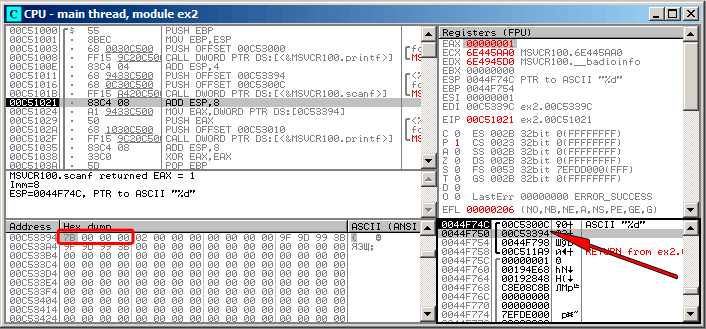
\includegraphics[scale=\FigScale]{patterns/04_scanf/2_global/ex2_olly_1.png}
\caption{\olly: \RU{после исполнения \scanf}\EN{after \scanf execution}}
\label{fig:scanf_ex2_olly_1}
\end{figure}

\RU{Переменная хранится в сегменте данных.}
\EN{The variable is located in the data segment.}
\RU{Кстати, после исполнения инструкции \PUSH (заталкивающей адрес $x$) адрес появится в стеке, 
и на этом элементе можно нажать правой кнопкой, выбрать \q{Follow in dump}.}
\EN{After the \PUSH instruction (pushing the address of $x$) gets executed, 
the address appears in the stack window. Right-click on that row and select \q{Follow in dump}.}
\RU{И в окне памяти слева появится эта переменная.}
\EN{The variable will appear in the memory window on the left.}

\RU{После того как в консоли введем 123, здесь появится}\EN{After we have entered 123 in the console,} 
\TT{0x7B}\EN{ appears in the memory window (see the highlighted screenshot regions)}.

\RU{Почему самый первый байт это}\EN{But why is the first byte} \TT{7B}?
\RU{По логике вещей, здесь должно было бы быть}\EN{Thinking logically,} \TT{00 00 00 7B}\EN{ should be
there}.
\RU{Это называется}\EN{The cause for this is referred as } \gls{endianness}, \RU{и в x86 принят формат }\EN{and x86 uses }\IT{little-endian}.
\RU{Это означает, что в начале записывается самый младший байт, а заканчивается самым старшим байтом}%
\EN{This implies that the lowest byte is written first, and the highest written last}.
\RU{Больше об этом}\EN{Read more about it at}: \myref{sec:endianness}.

\RU{Позже из этого места в памяти 32-битное значение загружается в \EAX и передается в}
\EN{Back to the example, the 32-bit value is loaded from this memory address into \EAX and passed to} \printf.

\RU{Адрес переменной $x$ в памяти}\EN{The memory address of $x$ is} \TT{0x00C53394}.

\clearpage
\RU{В \olly{} мы можем посмотреть карту памяти процесса (Alt-M) и увидим, что этот адрес
внутри PE-сегмента \TT{.data} нашей программы}%
\EN{In \olly we can review the process memory map (Alt-M)
and we can see that this address is inside the \TT{.data} PE-segment of our program}:

\begin{figure}[H]
\centering
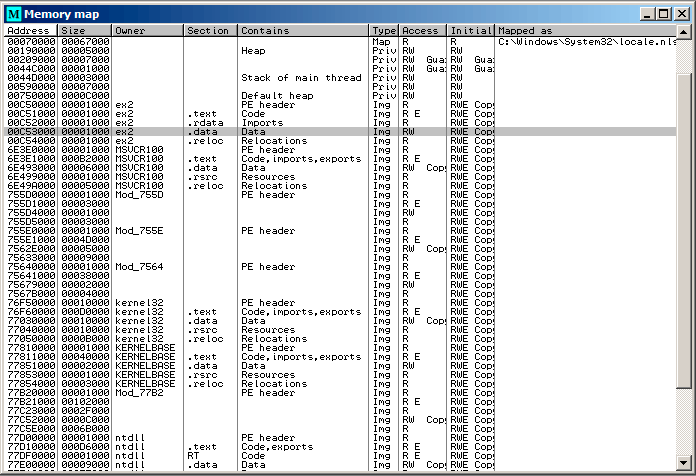
\includegraphics[scale=\FigScale]{patterns/04_scanf/2_global/ex2_olly_2.png}
\caption{\olly: \RU{карта памяти процесса}\EN{process memory map}}
\label{fig:scanf_ex2_olly_2}
\end{figure}

\fi

\ifdefined\IncludeGCC
\subsection{GCC: x86}

\index{ELF}
\RU{В Linux всё почти также. За исключением того, что если значение \TT{x} не определено, 
то эта переменная будет находится в сегменте \TT{\_bss}.
В \ac{ELF} этот сегмент имеет такие атрибуты:}
\EN{The picture in Linux is near the same, with the difference that the uninitialized variables are located in the \TT{\_bss} segment. 
In \ac{ELF} file this segment has the following attributes:}

\begin{lstlisting}
; Segment type: Uninitialized
; Segment permissions: Read/Write
\end{lstlisting}

\RU{Ну а если сделать статическое присвоение этой переменной какого-либо
значения, например, 10, то она будет находится 
в сегменте \TT{\_data},
это сегмент с такими атрибутами:}
\EN{If you, however, initialise the variable with some value e.g. 10, 
it is to be placed in the \TT{\_data} segment, which has the following attributes:}

\begin{lstlisting}
; Segment type: Pure data
; Segment permissions: Read/Write
\end{lstlisting}
\fi

\subsection{MSVC: x64}

\lstinputlisting[caption=MSVC 2012 x64]{patterns/04_scanf/2_global/ex2_MSVC_x64.asm.\LANG}

\RU{Почти такой же код как и в}\EN{The code is almost the same as in} x86.
\RU{Обратите внимание что для \TT{scanf()} адрес переменной $x$ передается
при помощи инструкции \LEA, а во второй \printf передается само значение переменной при помощи \MOV}
\EN{Please note that the address of the $x$ variable is passed to \TT{scanf()} using a \LEA instruction,
while the variable's value is passed to the second \printf using a \MOV instruction}.
\TT{DWORD PTR}\RU{\EMDASH{}это часть языка ассемблера (не имеющая отношения к машинным кодам) 
показывающая, что тип переменной в памяти именно 32-битный, 
и инструкция \MOV должна быть здесь закодирована соответственно}\EN{ is a part of the assembly language (no relation to the machine code), indicating that the variable data size is 32-bit and the \MOV instruction
has to be encoded accordingly}.

\ifdefined\IncludeARM
\subsection{ARM: \OptimizingKeilVI (\ThumbMode)}

\begin{lstlisting}
.text:00000000 ; Segment type: Pure code
.text:00000000                 AREA .text, CODE
...
.text:00000000 main
.text:00000000                 PUSH    {R4,LR}
.text:00000002                 ADR     R0, aEnterX     ; "Enter X:\n"
.text:00000004                 BL      __2printf
.text:00000008                 LDR     R1, =x
.text:0000000A                 ADR     R0, aD          ; "%d"
.text:0000000C                 BL      __0scanf
.text:00000010                 LDR     R0, =x
.text:00000012                 LDR     R1, [R0]
.text:00000014                 ADR     R0, aYouEnteredD___ ; "You entered %d...\n"
.text:00000016                 BL      __2printf
.text:0000001A                 MOVS    R0, #0
.text:0000001C                 POP     {R4,PC}
...
.text:00000020 aEnterX         DCB "Enter X:",0xA,0    ; DATA XREF: main+2
.text:0000002A                 DCB    0
.text:0000002B                 DCB    0
.text:0000002C off_2C          DCD x                   ; DATA XREF: main+8
.text:0000002C                                         ; main+10
.text:00000030 aD              DCB "%d",0              ; DATA XREF: main+A
.text:00000033                 DCB    0
.text:00000034 aYouEnteredD___ DCB "You entered %d...",0xA,0 ; DATA XREF: main+14
.text:00000047                 DCB 0
.text:00000047 ; .text         ends
.text:00000047
...
.data:00000048 ; Segment type: Pure data
.data:00000048                 AREA .data, DATA
.data:00000048                 ; ORG 0x48
.data:00000048                 EXPORT x
.data:00000048 x               DCD 0xA                 ; DATA XREF: main+8
.data:00000048                                         ; main+10
.data:00000048 ; .data         ends
\end{lstlisting}

\RU{Итак, переменная \TT{x} теперь глобальная, и она расположена, почему-то, в другом сегменте, а именно сегменте данных}
\EN{So, the \TT{x} variable is now global and for this reason located in another segment, namely the data segment} (\IT{.data}).
\RU{Можно спросить, почему текстовые строки расположены в сегменте кода (\IT{.text}), а \TT{x} нельзя было разместить тут же?}
\EN{One could ask, why are the text strings located in the code segment (\IT{.text}) and \TT{x} is located right here?}
\RU{Потому что эта переменная, и как следует из определения, она может меняться. И может быть, меняться часто.}
\EN{Because it is a variable and by definition its value could change. Moreover it could possibly change often.}
\RU{Ну а текстовые строки имеют тип констант, они не будут меняться, поэтому они располагаются в сегменте \IT{.text}.}
\EN{While text strings has constant type, they will not be changed, so they are located in the \IT{.text} segment.}
\index{\RAM}
\index{\ROM}
\RU{Сегмент кода иногда может быть расположен в ПЗУ микроконтроллера (не забывайте, 
мы сейчас имеем дело с embedded-микроэлектроникой, где дефицит памяти~--- обычное дело),
а изменяемые переменные~--- в ОЗУ.}
\EN{The code segment might sometimes be located in a \ac{ROM} chip (remember, we now deal
with embedded microelectronics, and memory scarcity is common here), and changeable 
variables~---in \ac{RAM}.}
\RU{Хранить в ОЗУ неизменяемые данные, когда в наличии есть ПЗУ, не экономно.}
\EN{It is not very economical to store constant variables in RAM when you have ROM.}
\RU{К тому же, сегмент данных в ОЗУ с константами нужно инициализировать перед работой,
ведь, после включения ОЗУ, очевидно, она содержит в себе случайную информацию.}
\EN{Furthermore, constant variables in RAM must be initialized, because after powering on, the RAM, obviously, contains random information.}

\index{\RU{Компоновщик}\EN{Linker}}
\RU{Далее мы видим в сегменте кода хранится указатель на переменную \TT{x} (\TT{off\_2C}) и 
все операции с переменной происходят через этот указатель.}
\EN{Moving forward, we see a pointer to the \TT{x} (\TT{off\_2C}) variable in the code segment, and that all
operations with the variable occur via this pointer.}
\RU{Это связано с тем, что переменная \TT{x} может быть расположена где-то довольно далеко от 
данного участка кода, так что её адрес нужно сохранить в непосредственной близости к этому коду.}
\EN{That is because the \TT{x} variable could be located somewhere far from this particular code fragment, so its address
must be saved somewhere in close proximity to the code.}
\index{ARM!\Instructions!LDR}
\RU{Инструкция \TT{LDR} в Thumb-режиме может адресовать только переменные в пределах вплоть 
до 1020 байт от своего местоположения.}
\EN{The \TT{LDR} instruction in Thumb mode can only address variables in a range of 1020 bytes from its location, }
\RU{Эта же инструкция в ARM-режиме~--- переменные в пределах $\pm{}4095$ байт.}
\EN{and in in ARM-mode~---variables in range of $\pm{}4095$ bytes.}
\RU{Таким образом,
адрес глобальной переменной \TT{x} нужно расположить в непосредственной близости, ведь нет никакой гарантии, 
что компоновщик\footnote{linker в англоязычной литературе} сможет разместить саму переменную где-то рядом, 
она может быть даже в другом чипе памяти!}
\EN{And so the address of the \TT{x} variable
must be located somewhere in close proximity, because there is no guarantee that the linker would be able to accommodate the variable somewhere nearby the code, it may well be even in an external memory chip!}

\index{\CLanguageElements!const}
\index{\ROM}
\RU{Ещё одна вещь: если переменную объявить как \IT{const}, то компилятор Keil разместит её в 
сегменте \TT{.constdata}.}
\EN{One more thing: if a variable is declared as \IT{const}, the Keil compiler allocates it in 
the \TT{.constdata} segment.}
\RU{Должно быть, впоследствии компоновщик и этот сегмент сможет разместить в ПЗУ вместе
с сегментом кода.}
\EN{Perhaps, thereafter, the linker could place this segment in ROM too, along with the code segment.}

\subsection{ARM64}

\lstinputlisting[caption=\NonOptimizing GCC 4.9.1 ARM64,numbers=left]{patterns/04_scanf/2_global/ARM64_GCC491_O0.s.\LANG}

\index{ARM!\Instructions!ADRP/ADD pair}
\RU{Теперь $x$ это глобальная переменная, и её адрес вычисляется при помощи пары инструкций ADRP/ADD 
(строки 21 и 25).}
\EN{In this case the $x$ variable is declared as global and its address is calculated using 
the ADRP/ADD instruction pair (lines 21 and 25).}

\fi
\ifdefined\IncludeMIPS
\subsection{MIPS}

\subsubsection{\EN{Uninitialized global variable}\RU{Неинициализированная глобальная переменная}}

\RU{Так что теперь переменная $x$ глобальная.}
\EN{So now the $x$ variable is global.}
\RU{Сделаем исполняемый файл вместо объектного и загрузим его в \IDA.}
\EN{Let's compile to executable file rather than object file and load it into \IDA.}
\RU{IDA показывает присутствие переменной $x$ в ELF-секции .sbss (помните о \q{Global Pointer}? \myref{MIPS_GP}),
так как переменная не инициализируется в самом начале.}
\EN{IDA displays the $x$ variable in the .sbss ELF section (remember the \q{Global Pointer}? \myref{MIPS_GP}),
since the variable is not initialized at the start.}

\lstinputlisting[caption=\Optimizing GCC 4.4.5 (IDA)]{patterns/04_scanf/2_global/MIPS/O3_IDA.lst.\LANG}

\RU{IDA уменьшает количество информации, так что сделаем также листинг используя objdump и добавим туда свои комментарии:}%
\EN{IDA reduces the amount of information, so we'll also do a listing using objdump and comment it:}

\lstinputlisting[caption=\Optimizing GCC 4.4.5 (objdump),numbers=left]{patterns/04_scanf/2_global/MIPS/O3_objdump.txt.\LANG}

\RU{Теперь мы видим, как адрес переменной $x$ берется из буфера 64KiB, используя GP и прибавление
к нему отрицательного смещения (строка 18).}
\EN{Now we see the $x$ variable address is read from a 64KiB data buffer using GP and adding
negative offset to it (line 18).}
\RU{И даже более того: адреса трех внешних функций, используемых в нашем примере (\puts, \scanf, \printf)
также берутся из буфера 64KiB используя GP (строки 9, 16 и 26).}
\EN{More than that, the addresses of the three external functions  which are used in our example (\puts, \scanf, \printf), are also read from the 64KiB global data buffer using GP (lines 9, 16 and 26).}
\RU{GP указывает на середину буфера, так что такие смещения могут нам подсказать, что адреса всех трех функций,
а также адрес переменной $x$ расположены где-то в самом начале буфера.}
\EN{GP points to the middle of the buffer, and such offset suggests that all three function's addresses,
and also the address of the $x$ variable, are all stored somewhere at the beginning of that buffer.}
\RU{Действительно, ведь наш пример крохотный}\EN{That make sense, because our example is tiny}.

\index{MIPS!\Pseudoinstructions!MOVE}
\index{MIPS!\Pseudoinstructions!NOP}
\RU{Ещё нужно отметить что функция заканчивается двумя \ac{NOP}-ами (\TT{MOVE \$AT,\$AT}~--- 
это холостая инструкция), чтобы выровнять начало следующей функции по 16-байтной границе.}
\EN{Another thing worth mentioning is that the function ends with two \ac{NOP}s (\TT{MOVE \$AT,\$AT} --- 
an idle instruction), in order to align next function's start on 16-byte boundary.}

\subsubsection{\RU{Инициализированная глобальная переменная}\EN{Initialized global variable}}

\RU{Немного изменим наш пример и сделаем, чтобы у $x$ было значение по умолчанию:}
\EN{Let's alter our example by giving the $x$ variable a default value:}

\lstinputlisting{patterns/04_scanf/2_global/default_value.c.\LANG}

\RU{Теперь IDA показывает что переменная $x$ располагается в секции .data:}
\EN{Now IDA shows that the $x$ variable is residing in the .data section:}

\lstinputlisting[caption=\Optimizing GCC 4.4.5 (IDA)]{patterns/04_scanf/2_global/MIPS/O3_IDA_init.lst.\LANG}

\RU{Почему не .sdata? Может быть, нужно было указать какую-то опцию в GCC?}
\EN{Why not .sdata? Perhaps that this depends on some GCC option?}
\RU{Тем не менее, $x$ теперь в .data, а это уже общая память и мы можем посмотреть как происходит
работа с переменными там.}
\EN{Nevertheless, now $x$ is in .data, which is a general memory area, and we can take a look
how to work with variables there.}

\index{MIPS!\Instructions!LUI}
\index{MIPS!\Instructions!ADDIU}
\RU{Адрес переменной должен быть сформирован парой инструкций.}
\EN{The variable's address must be formed using a pair of instructions.}
\RU{В нашем случае это LUI (\q{Load Upper Immediate}~--- загрузить старшие 16 бит) и 
ADDIU (\q{Add Immediate Unsigned Word}~--- прибавить значение).}
\EN{In our case those are LUI (\q{Load Upper Immediate}) and ADDIU (\q{Add Immediate Unsigned Word}).}

\RU{Вот так же листинг сгенерированный objdump-ом для лучшего рассмотрения:}
\EN{Here is also the objdump listing for close inspection:}

\lstinputlisting[caption=\Optimizing GCC 4.4.5 (objdump)]{patterns/04_scanf/2_global/MIPS/O3_objdump_init.txt.\LANG}

\index{MIPS!\Instructions!LUI}
\index{MIPS!\Instructions!ADDIU}
\index{MIPS!\Instructions!LW}
\RU{Адрес формируется используя LUI и ADDIU, но старшая часть адреса
всё ещё в регистре \$S0, и можно закодировать смещение в инструкции LW (\q{Load Word}), так что одной
LW достаточно для загрузки значения из переменной и передачи его в \printf.}
\EN{We see that the address is formed using LUI and ADDIU, but the high part of address is still in
the \$S0 register, and it is possible to encode the offset in a LW (\q{Load Word}) instruction, so one single LW is enough 
to load a value from the variable and pass it to \printf.}

\RU{Регистры хранящие временные данные имеют префикс T-, но здесь есть также регистры с префиксом S-,
содержимое которых должно быть сохранено в других функциях (т.е. \q{saved}).}
\EN{Registers holding temporary data are prefixed with T-, but here we also see some prefixed with S-, 
the contents of which is need to be preserved before use in other functions (i.e., \q{saved}).}
% FIXME:
% This needs to be clarified a bit, e.g. "the registers need to be preserved if a function is called and it wants to use them
\RU{Вот почему \$S0 был установлен по адресу 0x4006cc и затем был использован по адресу 0x4006e8
после вызова \scanf.}
\EN{That is why the value of \$S0 was set at address 0x4006cc and was used again
at address 0x4006e8, after the \scanf call. }
\RU{Функция \scanf не изменяет это значение.}\EN{The \scanf function does not change its value.}

% TODO non-optimized example?

\fi

\section{\RU{Проверка результата scanf()}\EN{scanf() result checking}}

\RU {Как уже было упомянуто, использовать \scanf в наше время слегка старомодно. 
Но если уж жизнь заставила этим заниматься, нужно хотя бы проверять, сработал ли \scanf 
правильно или пользователь ввел вместо числа что-то другое, что \scanf не смог трактовать как число.}%
\EN{As was noted before, it is slightly old-fashioned to use \scanf today. 
But if we have to, we need to at least check if \scanf finishes correctly without an error.}

\lstinputlisting{patterns/04_scanf/3_checking_retval/ex3.c}

\RU{По стандарту,}\EN{By standard, the} 
\scanf\footnote{scanf, wscanf: \href{http://go.yurichev.com/17255}{MSDN}} 
\RU{возвращает количество успешно полученных значений.}
\EN{function returns the number of fields it has successfully read.}

\RU{В нашем случае, если всё успешно и пользователь ввел таки некое число, \scanf вернет 1. 
А если нет, то 0 (или \ac{EOF}).} 
\EN{In our case, if everything goes fine and the user enters a number 
\scanf returns 1, or in case of error (or \ac{EOF}) --- 0.}

\RU{Добавим код, проверяющий результат \scanf и в случае ошибки он сообщает пользователю что-то другое.}%
\EN{Let's add some C code to check the \scanf return value and print error message in case of an error.}

\RU{Это работает предсказуемо}\EN{This works as expected}:

\begin{lstlisting}
C:\...>ex3.exe
Enter X:
123
You entered 123...

C:\...>ex3.exe
Enter X:
ouch
What you entered? Huh?
\end{lstlisting}

% subsections
\subsection{MSVC: x86}

\RU{Вот что выходит на ассемблере}\EN{Here is what we get in the assembly output} (MSVC 2010):

\lstinputlisting{patterns/04_scanf/3_checking_retval/ex3_MSVC_x86.asm}

\index{x86!\Registers!EAX}
\RU{Для того чтобы вызывающая функция имела доступ к результату вызываемой функции, 
вызываемая функция (в нашем случае \scanf) оставляет это значение в регистре \EAX.}
\EN{The \gls{caller} function (\main) needs the \gls{callee} function (\scanf) result, 
so the \gls{callee} returns it in the \EAX register.}

\index{x86!\Instructions!CMP}
\RU{Мы проверяем его инструкцией \TT{CMP EAX, 1} (\IT{CoMPare}), то есть 
сравниваем значение в \EAX с 1.}
\EN{We check it with the help of the instruction \TT{CMP EAX, 1} (\IT{CoMPare}).
In other words, we compare the value in the \EAX register with 1.} 

\index{x86!\Instructions!JNE}
\RU{Следующий за инструкцией \CMP: условный переход \JNE. 
Это означает \IT{Jump if Not Equal}, то есть условный переход \IT{если не равно}.}
\EN{A \JNE conditional jump follows the \CMP instruction. \JNE stands for \IT{Jump if Not Equal}.}

\RU{Итак, если \EAX не равен 1, то \JNE заставит \ac{CPU} перейти 
по адресу указанном в операнде \JNE, у нас это \TT{\$LN2@main}.}
\EN{So, if the value in the \EAX register is not equal to 1, 
the \ac{CPU} will pass the execution to the 
address mentioned in the \JNE operand, in our case \TT{\$LN2@main}.}
\RU{Передав управление по этому адресу, \ac{CPU} начнет исполнять вызов \printf с 
аргументом \TT{What you entered? Huh?}.}
\EN{Passing the control to this address results in the \ac{CPU} executing \printf 
with the argument \TT{What you entered? Huh?}.}
\RU{Но если всё нормально, перехода не случится и исполнится другой \printf с двумя аргументами: 
\TT{'You entered \%d...'} и значением переменной \TT{x}.}
\EN{But if everything is fine, the conditional jump is not be be taken, and another \printf call 
is to be executed, with two arguments: \TT{'You entered \%d...'} and the value of \TT{x}. }

\index{x86!\Instructions!XOR}
\index{\CLanguageElements!return}
\RU{Для того чтобы после этого вызова не исполнился сразу второй вызов \printf, 
после него есть инструкция \JMP, безусловный переход, который отправит процессор на место 
после второго \printf и перед инструкцией \TT{XOR EAX, EAX}, которая реализует \TT{return 0}.}
\EN{Since in this case the second \printf has not to be executed, there is a \JMP preceding it (unconditional jump). 
It passes the control to the point after the second \printf and just before the \TT{XOR EAX, EAX} instruction, which implements \TT{return 0}.}

\index{x86!\Registers!\Flags}
\RU{Итак, можно сказать что в подавляющих случаях сравнение какой-либо переменной с чем-то другим 
происходит при помощи пары инструкций \CMP и \Jcc, где \IT{cc} это \IT{condition code}.}
\EN{So, it could be said that comparing a value with another is \IT{usually} implemented
by \CMP/\Jcc instruction pair, where \IT{cc} is \IT{condition code}.}
\RU{\CMP сравнивает два значения и выставляет 
флаги процессора\footnote{См. также о флагах x86-процессора: \href{http://go.yurichev.com/17120}{wikipedia}.}.}
\EN{\CMP compares two values and sets 
processor flags\footnote{x86 flags, see also: \href{http://go.yurichev.com/17120}{wikipedia}.}.}
\RU{\Jcc проверяет нужные ему флаги и выполняет переход по указанному адресу (или не выполняет).}
\EN{\Jcc checks those flags and decides to either pass the control to the specified address or not.}

\index{x86!\Instructions!CMP}
\index{x86!\Instructions!SUB}
\label{CMPandSUB}
\RU{Но на самом деле, как это не парадоксально поначалу звучит, \CMP это почти то же самое что и 
инструкция \SUB, которая отнимает числа одно от другого.}
\EN{This could sound paradoxical, but the \CMP instruction is in fact \SUB (subtract).}
\RU{Все арифметические инструкции также выставляют флаги в соответствии с результатом, не только \CMP.}
\EN{All arithmetic instructions set processor flags, not just \CMP.}
\RU{Если мы сравним 1 и 1, от единицы отнимется единица, получится 0, и выставится флаг 
\ZF (\IT{zero flag}), означающий, что последний полученный результат был 0.}
\EN{If we compare 1 and 1, $1-1$ is 0 so the \ZF flag would be set (meaning that the last result was 0).}
\RU{Ни при каких других значениях \EAX, флаг \ZF не может быть выставлен, кроме тех, когда операнды равны друг другу.}
\EN{In no other circumstances \ZF can be set, except when the operands are equal.}
\index{x86!\Instructions!JNE}
\index{x86!\Registers!ZF}
\RU{Инструкция \JNE проверяет только флаг \ZF, и совершает переход только если флаг не поднят. 
Фактически, \JNE это синоним инструкции \JNZ (\IT{Jump if Not Zero}).}
\EN{\JNE checks only the \ZF flag and jumps only if it is not set. 
\JNE is in fact a synonym for \JNZ (\IT{Jump if Not Zero}).}
\RU{Ассемблер транслирует обе инструкции в один и тот же опкод.}
\EN{Assembler translates both \JNE and \JNZ instructions into the same opcode.}
\RU{Таким образом, можно \CMP заменить на \SUB и всё будет работать также, но разница в том, что \SUB 
всё-таки испортит значение в первом операнде. \CMP это \IT{SUB без сохранения результата, но изменяющая флаги}.}
\EN{So, the \CMP instruction can be replaced with a \SUB instruction 
and almost everything will be fine,
with the difference that \SUB alters the value of the first operand.
\CMP is \IT{SUB without saving the result, but affecting flags}.}

\ifx\LITE\undefined
\subsection{MSVC: x86: IDA}

\index{IDA}
\RU{Наверное, уже пора делать первые попытки анализа кода в \IDA}%
\EN{It is time to run \IDA and try to do something in it}.
\RU{Кстати, начинающим полезно компилировать в MSVC с ключом \TT{/MD}, что означает что все эти стандартные
функции не будут скомпонованы с исполняемым файлом, а будут импортироваться из файла \TT{MSVCR*.DLL}.}
\EN{By the way, for beginners it is good idea to use \TT{/MD} option in MSVC, which means that all these
standard functions are not be linked with the executable file, 
but are to be imported from the \TT{MSVCR*.DLL} file instead.}
\RU{Так будет легче увидеть, где какая стандартная функция используется.}
\EN{Thus it will be easier to see which standard function are used and where.}

\RU{Анализируя код в \IDA, очень полезно делать пометки для себя (и других).}
\EN{While analysing code in \IDA, it is very helpful to leave notes for oneself (and others)}.
\RU{Например, разбирая этот пример, мы сразу видим, что \TT{JNZ} срабатывает в случае ошибки.}
\EN{In instance, analysing this example, 
we see that \TT{JNZ} is to be triggered in case of an error.}
\RU{Можно навести курсор на эту метку, нажать \q{n} и переименовать метку в \q{error}.}
\EN{So it is possible to move the cursor to the label, press \q{n} and rename it to \q{error}.}
\RU{Ещё одну метку}\EN{Create another label}\EMDASH{}\RU{в}\EN{into} \q{exit}.
\RU{Вот как у меня получилось в итоге}\EN{Here is my result}:

\lstinputlisting{patterns/04_scanf/3_checking_retval/ex3.lst}

\RU{Так понимать код становится чуть легче}\EN{Now it is slightly easier to understand the code}.
\RU{Впрочем, меру нужно знать во всем и комментировать каждую инструкцию не стоит.}
\EN{However, it is not a good idea to comment on every instruction.}

% FIXME draw button?
\RU{В \IDA также можно скрывать части функций: нужно выделить скрываемую часть, нажать \q{--} на цифровой клавиатуре и ввести текст}
\EN{You could also hide(collapse) parts of a function in \IDA.
To do that mark the block, then press \q{--} on the numerical pad and enter the text to be displayed instead}.

\RU{Скроем две части и придумаем им названия}\EN{Let's hide two blocks and give them names}:

\lstinputlisting{patterns/04_scanf/3_checking_retval/ex3_2.lst}

% FIXME draw button?
\RU{Раскрывать скрытые части функций можно при помощи \q{+} на цифровой клавиатуре}
\EN{To expand previously collapsed parts of the code, use \q{+} on the numerical pad}.

\clearpage
\RU{Нажав \q{пробел}, мы увидим, как \IDA может представить функцию в виде графа}\EN{By pressing \q{space},
we can see how \IDA represents a function as a graph}:

\begin{figure}[H]
\centering
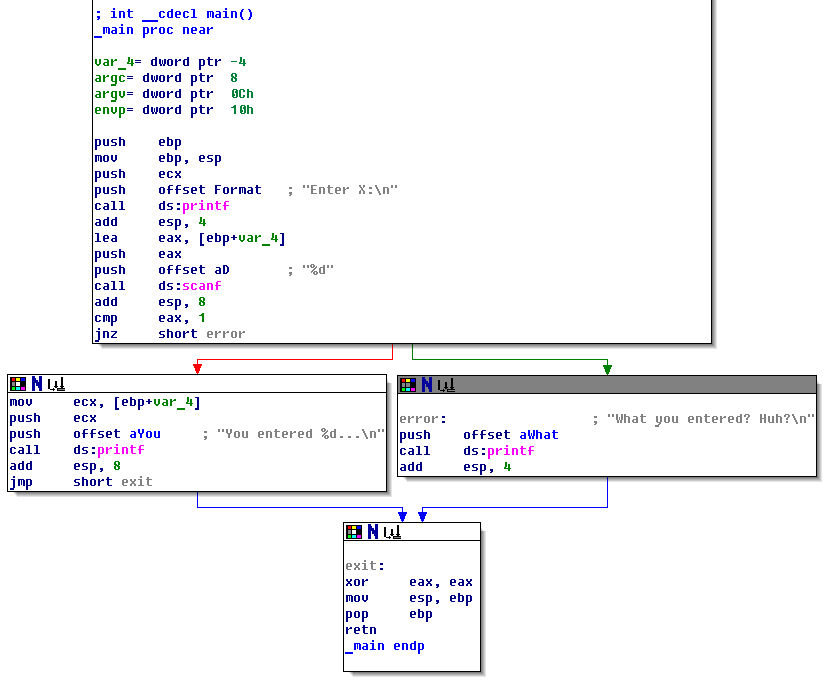
\includegraphics[scale=\FigScale]{patterns/04_scanf/3_checking_retval/IDA.png}
\caption{\RU{Отображение функции в IDA в виде графа}\EN{Graph mode in IDA}}
\label{fig:ex3_IDA_1}
\end{figure}

\RU{После каждого условного перехода видны две стрелки: зеленая и красная}\EN{There are two arrows
after each conditional jump: green and red}.
\RU{Зеленая ведет к тому блоку, который исполнится если переход сработает, 
а красная~--- если не сработает.}
\EN{The green arrow points to the block which executes if the jump is triggered, 
and red if otherwise.}

\clearpage
\RU{В этом режиме также можно сворачивать узлы и давать им названия}
\EN{It is possible to fold nodes in this mode and give them names as well} (\q{group nodes}).
\RU{Сделаем это для трех блоков}\EN{Let's do it for 3 blocks}:

\begin{figure}[H]
\centering
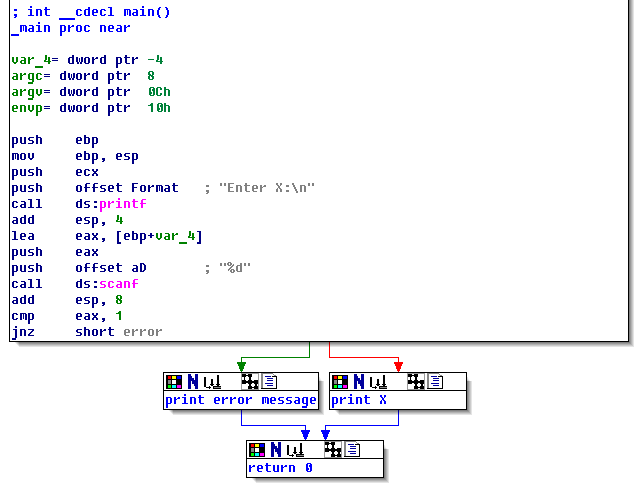
\includegraphics[scale=\FigScale]{patterns/04_scanf/3_checking_retval/IDA2.png}
\caption{\RU{Отображение в IDA в виде графа с тремя свернутыми блоками}\EN{Graph mode in IDA with 3 nodes folded}}
\label{fig:ex3_IDA_2}
\end{figure}

\RU{Всё это очень полезно делать}\EN{That is very useful}.
\RU{Вообще, очень важная часть работы реверсера (да и любого исследователя) состоит в том, чтобы уменьшать количество имеющейся информации.}
\EN{It could be said that a very important part of the reverse engineers' job (and any other researcher as well) is to reduce the amount of information they deal with.}
\fi

\ifdefined\IncludeOlly
\clearpage
\subsection{MSVC: x86 + \olly}

\RU{Попробуем в \olly немного хакнуть программу и сделать вид, что \scanf срабатывает всегда без ошибок.}
\EN{Let's try to hack our program in \olly, forcing it to think \scanf always works without error.}

\RU{Когда в \scanf передается адрес локальной переменной, изначально в этой переменной
находится некий мусор. В данном случае это}\EN{When an address of a local variable is passed into \scanf,
the variable initially contains some random garbage, in this case} \TT{0x6E494714}:

\begin{figure}[H]
\centering
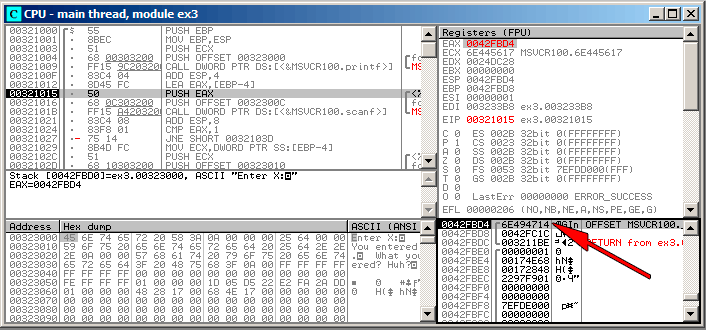
\includegraphics[scale=\FigScale]{patterns/04_scanf/3_checking_retval/olly_1.png}
\caption{\olly: \RU{передача адреса переменной в}\EN{passing variable address into} \scanf}
\label{fig:scanf_ex3_olly_1}
\end{figure}

\clearpage
\RU{Когда}\EN{While} \scanf \RU{запускается, вводим в консоли что-то непохожее на число, например}
\EN{executes, in the console we enter something that is definitely not a number, like} \q{asdasd}.
\scanf \RU{заканчивается с 0 в}\EN{finishes with 0 in} \EAX, \RU{что означает, что произошла ошибка}%
\EN{which indicates that an error has occurred}:

\begin{figure}[H]
\centering
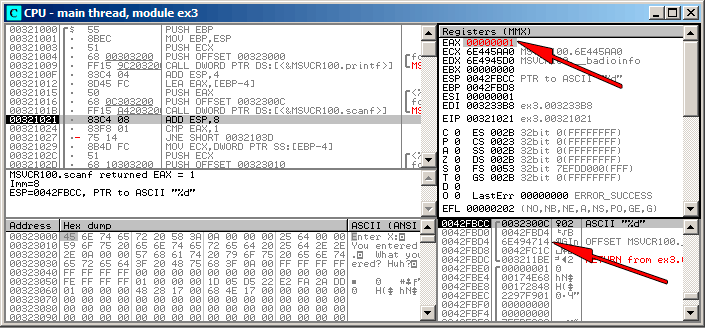
\includegraphics[scale=\FigScale]{patterns/04_scanf/3_checking_retval/olly_2.png}
\caption{\olly: \scanf \RU{закончился с ошибкой}\EN{returning error}}
\label{fig:scanf_ex3_olly_2}
\end{figure}

\RU{Вместе с этим мы можем посмотреть на локальную переменную в стеке~--- она не изменилась.}
\EN{We can also check the local variable in the stack and note that it has not changed.}
\RU{Действительно, ведь что туда записала бы функция \scanf}\EN{Indeed, what would \scanf write there}?
\RU{Она не делала ничего кроме возвращения нуля}\EN{It simply did nothing except returning zero}.

\RU{Попробуем ещё немного \q{хакнуть} нашу программу}\EN{Let's try to \q{hack} our program}.
\RU{Щелкнем правой кнопкой на}\EN{Right-click on} \EAX, \RU{там, в числе опций, будет также}
\EN{Among the options there is} \q{Set to 1}.
\RU{Это нам и нужно}\EN{This is what we need}.

\RU{В \EAX теперь 1, последующая проверка пройдет как надо, и \printf выведет значение переменной
из стека.}
\EN{We now have 1 in \EAX, so the following check is to be executed as intended, 
and \printf will print the value of the variable in the stack.}

\RU{Запускаем (F9) и видим в консоли следующее:}
\EN{When we run the program (F9) we can see the following in the console window:}

\begin{figure}[H]
\centering
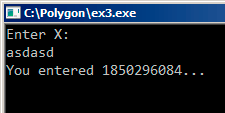
\includegraphics[scale=\FigScale]{patterns/04_scanf/3_checking_retval/olly_3.png}
\caption{\RU{консоль}\EN{console window}}
\end{figure}

\RU{Действительно}\EN{Indeed}, 1850296084 \RU{это десятичное представление числа в стеке}
\EN{is a decimal representation of the number in the stack} (\TT{0x6E494714})!

\fi

\clearpage
\subsection{MSVC: x86 + Hiew}
\index{Hiew}

\RU{Это ещё может быть и простым примером исправления исполняемого файла}\EN{This can also be used as 
a simple example of executable file patching}.
\RU{Мы можем попробовать исправить его таким образом, что программа всегда будет выводить числа,
вне зависимости от ввода}\EN{We may try to patch the executable so the program would always 
print the input, no matter what we enter}.

\RU{Исполняемый файл скомпилирован с импортированием функций из}\EN{Assuming that the 
executable is compiled against external} \TT{MSVCR*.DLL} (\RU{т.е. с опцией}\EN{i.e., with} 
\TT{/MD}\EN{ option})\footnote{\RU{то, что ещё называют}\EN{that's what also called} \q{dynamic linking}}, 
\RU{поэтому мы можем отыскать функцию}\EN{we see the} \main \RU{в самом начале секции}\EN{function at the 
beginning of the} \TT{.text}\EN{ section}.
\RU{Откроем исполняемый файл в Hiew, найдем самое начало секции}\EN{Let's open the executable in Hiew and 
find the beginning of the} \TT{.text}\EN{ section} (Enter, F8, F6, Enter, Enter).

\RU{Мы увидим следующее}\EN{We can see this}:

\begin{figure}[H]
\centering
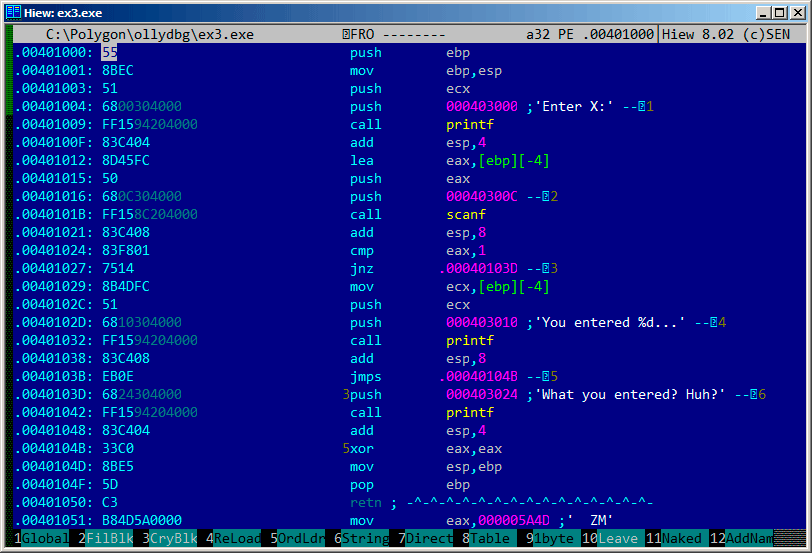
\includegraphics[scale=\FigScale]{patterns/04_scanf/3_checking_retval/hiew_1.png}
\caption{Hiew: \RU{функция }\main\EN{ function}}
\label{fig:scanf_ex3_hiew_1}
\end{figure}

Hiew \RU{находит}\EN{finds} \ac{ASCIIZ}\RU{-строки и показывает их, также как и имена импортируемых 
функций}\EN{ strings and displays them, as it does with the imported functions' names}.

\clearpage
\RU{Переведите курсор на адрес}\EN{Move the cursor to address} \TT{.00401027} 
(\RU{с инструкцией}\EN{where the} \TT{JNZ}\RU{, которую мы хотим заблокировать}\EN{ instruction, we 
have to bypass, is located}), \RU{нажмите}\EN{press} F3,
\RU{затем наберите}\EN{and then type} \q{9090}(\RU{ что означает два}\EN{, meaning two} \ac{NOP}\RU{-а}\EN{s}): 

\begin{figure}[H]
\centering
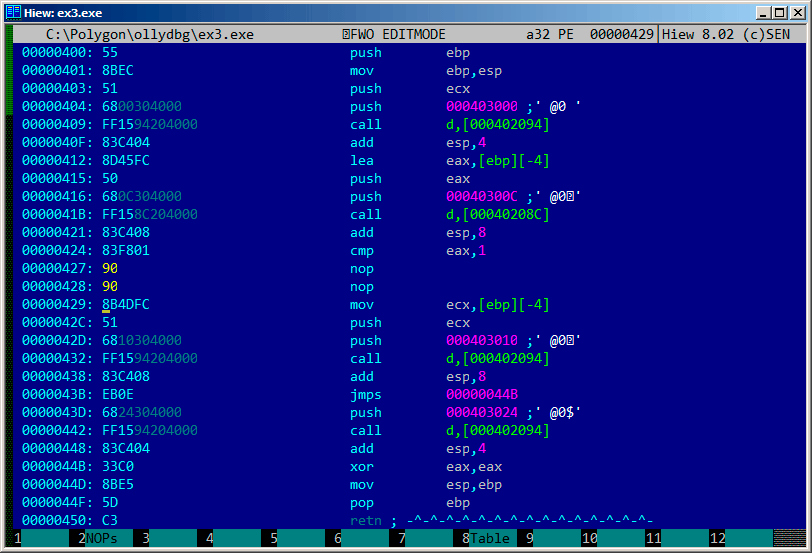
\includegraphics[scale=\FigScale]{patterns/04_scanf/3_checking_retval/hiew_2.png}
\caption{Hiew: \RU{замена}\EN{replacing} \TT{JNZ} \RU{на два}\EN{with two} \ac{NOP}\RU{-а}\EN{s}}
\label{fig:scanf_ex3_hiew_2}
\end{figure}

\RU{Затем}\EN{Then press} F9 (update). \RU{Теперь исполняемый файл записан на диск. Он будет вести себя
так, как нам надо.}\EN{Now the executable is saved to the disk. It will behave as we wanted.}

\RU{Два}\EN{Two} \ac{NOP}\RU{-а}\EN{s} \RU{возможно, не так эстетично, как могло бы быть}\EN{are probably 
not the most \ae{}sthetic approach}.
\RU{Другой способ изменить инструкцию это записать 0 во второй байт опкода (смещение перехода),
так что}\EN{Another way to patch this instruction is to write just 0 to the second opcode byte (\gls{jump offset}), 
so that} \TT{JNZ} \RU{всегда будет переходить на следующую инструкцию}\EN{will always jump to 
the next instruction}.

\RU{Можно изменить и наоборот: первый байт заменить на \TT{EB}, второй байт (смещение перехода) не трогать.}
\EN{We could also do the opposite: replace first byte with \TT{EB} while not touching the second byte (\gls{jump offset}).}
\RU{Получится всегда срабатывающий безусловный переход}\EN{We would get an unconditional jump that is always triggered}.
\RU{Теперь сообщение об ошибке будет выдаваться всегда, даже если мы ввели число.}
\EN{In this case the error message would be printed every time, no matter the input.}

\subsection{MSVC: x64}

\index{x86-64}
\RU{Так как здесь мы работаем с переменными типа \Tint, а они в x86-64 остались 32-битными, то мы здесь видим,
как продолжают использоваться регистры с префиксом \TT{E-}.}\EN{Since we work here with \Tint{}-typed variables,
which are still 32-bit in x86-64, we see how the 32-bit part of the registers (prefixed with \TT{E-}) 
are used here as well.}
\RU{Но для работы с указателями, конечно, используются 64-битные части регистров с префиксом \TT{R-}.}
\EN{While working with pointers, however, 64-bit register parts are used, prefixed with \TT{R-}.}

\lstinputlisting[caption=MSVC 2012 x64]{patterns/04_scanf/3_checking_retval/ex3_MSVC_x64.asm.\LANG}


\ifdefined\IncludeARM
\subsection{ARM}

\subsubsection{ARM: \OptimizingKeilVI (\ThumbMode)}

\lstinputlisting[caption=\OptimizingKeilVI (\ThumbMode)]{patterns/04_scanf/3_checking_retval/ex3_ARM_Keil_thumb_O3.asm}

\index{ARM!\Instructions!CMP}
\index{ARM!\Instructions!BEQ}
\RU{Здесь для нас есть новые инструкции: \CMP и \ac{BEQ}.}
\EN{The new instructions here are \CMP and \ac{BEQ}.}

\CMP \RU{аналогична той что в x86: она отнимает один аргумент от второго и сохраняет флаги.}
\EN{is analogous to the x86 instruction with the same name, it subtracts one of the arguments from the other and updates the conditional flags if needed.}
% TODO: в мануале ARM $op1 + NOT(op2) + 1$ вместо вычитания

\index{ARM!\Registers!Z}
\index{x86!\Instructions!JZ}
\ac{BEQ} \RU{совершает переход по другому адресу, 
если операнды при сравнении были равны, 
либо если результат последнего вычисления был 0, либо если флаг Z равен 1.}
\EN{jumps to another address if the operands were equal to each other, or,
if the result of the last computation was 0, or if the Z flag is 1.}
\RU{То же что и \JZ в}\EN{It behaves as \JZ in} x86.

\RU{Всё остальное просто: исполнение разветвляется на две ветки, затем они сходятся там, 
где в \Reg{0} записывается 0 как возвращаемое из функции значение и происходит выход из функции.}
\EN{Everything else is simple: the execution flow forks in two branches, then the branches
converge at the point
where 0 is written into the \Reg{0} as a function return value, and then the function ends.}

\subsubsection{ARM64}

\lstinputlisting[caption=\NonOptimizing GCC 4.9.1 ARM64,numbers=left]{patterns/04_scanf/3_checking_retval/ARM64_GCC491_O0.s.\LANG}

\index{ARM!\Instructions!CMP}
\index{ARM!\Instructions!Bcc}
\EN{Code flow in this case forks with the use of CMP/BNE (Branch if Not Equal) instructions pair.}
\RU{Исполнение здесь разветвляется, используя пару инструкций CMP/BNE (Branch if Not Equal: переход если не равно).}

\fi
\ifdefined\IncludeMIPS
\subsection{MIPS}

\lstinputlisting[caption=\Optimizing GCC 4.4.5 (IDA)]{patterns/04_scanf/3_checking_retval/MIPS_O3_IDA.lst}

\index{MIPS!\Instructions!BEQ}
\RU{\scanf возвращает результат своей работы в регистре \$V0 и он проверяется по адресу 0x004006E4
сравнивая значения в \$V0 и \$V1 (1 записан в \$V1 ранее, на 0x004006DC).}
\EN{\scanf returns the result of its work in register \$V0. It is checked at address 0x004006E4
by comparing the values in \$V0 with \$V1 (1 was stored in \$V1 earlier, at 0x004006DC).}
BEQ \EN{stands for}\RU{означает} \q{Branch Equal}\RU{ (переход если равно)}.
\RU{Если значения равны (т.е. в случае успеха), произойдет переход по адресу 0x0040070C.}
\EN{If the two values are equal (i.e., success), the execution jumps to address 0x0040070C.}

\fi

\ifdefined\IncludeExercises
\subsection{\Exercise}

\index{x86!\Instructions!Jcc}
\index{ARM!\Instructions!Bcc}
\EN{As we can see, the JNE/JNZ instruction can be easily replaced by the JE/JZ and vice versa 
(or BNE by BEQ and vice versa).}
\RU{Как мы можем увидеть, инструкцию JNE/JNZ можно вполне заменить на JE/JZ или наоборот 
(или BNE на BEQ и наоборот).}
\EN{But then the basic blocks must also be swapped.}\RU{Но при этом ещё нужно переставить базовые блоки местами.}
\EN{Try to do this in some of the examples.}\RU{Попробуйте сделать это в каком-нибудь примере.}
\fi


\section{\Exercises}

\subsection{\Exercise \#1}
\label{exercise_scanf_1}

\EN{This code, compiled in Linux x86-64 using GCC is crashing while execution (segmentation fault).
However, it works in Windows environment compiled by MSVC 2010 x86.
Why?}
\RU{Этот код, когда компилируется при помощи GCC в Linux x86-64, падает во время исполнения (segmentation fault).
Но он работает в среде Windows, когда скомпилирован при помощи MSVC 2010 x86.
Почему?}

\begin{lstlisting}
#include <string.h>
#include <stdio.h>

void alter_string(char *s)
{
        strcpy (s, "Goodbye!");
        printf ("Result: %s\n", s);
};

int main()
{
        alter_string ("Hello, world!\n");
};
\end{lstlisting}


\Answer{}: \myref{exercise_solutions_scanf_1}.

